\section{Background}\label{sec:background}
The NASA Viking missions in the 1970s were the first to successfully land on Mars, aiming to determine if life existed on the planet.
One experiment suggested the presence of life, but the results were ambiguous and inconclusive, and NASA was unable to repeat the experiment.
Nevertheless, these missions were deemed a monumental success and advanced our knowledge of the Martian environment~\cite{marsnasagov_vikings}.

Leveraging the knowledge gained from the Viking missions, NASA launched the \gls{mer} mission in 2003 to investigate whether Mars ever had the conditions to support life as we know it.
The mission landed two rovers, Spirit and Opportunity, on Mars in January 2004, and they quickly discovered clear evidence that water once flowed on Mars.
However, since water alone is not enough to support life, the next objective was to search for organic material as well~\cite{marsnasagov_observer, marsnasagov_spirit_opportunity}.

The Curiosity rover landed on Mars in August 2012 inside Gale Crater as part of the \gls{msl} mission with this very purpose.
Thanks to its sophisticated equipment, Curiosity was able to find evidence of past habitable environments on Mars based on chemical and mineral findings early in its mission~\cite{marsnasagov_msl}.

One of the instruments aboard the rover is the \gls{chemcam} instrument, which is a remote-sensing laser instrument used to gather \gls{libs} data from geological samples on Mars.
\gls{libs} is a technique that enables rapid analysis by using a laser to ablate and remove surface contaminants to expose the underlying material and generate a plasma plume from the now-exposed sample material~\cite{wiensChemcam2012}.
This plasma plume emits light that is captured through three distinct spectrometers to collect a series of spectral readings.
These spectra consist of emission lines that can be associated with the concentration of a specific element, and their intensity reflects the concentration of that element in the sample.
Consequently, a spectra serves as a complex, multi-dimensional fingerprint of the elemental composition of the examined geological samples~\cite{cleggRecalibrationMarsScience2017}.

\subsection{Baseline \& Replica}\label{sec:baseline_replica}
For analyzing Martian geological samples, the \gls{chemcam} team currently uses the \gls{moc} model~\cite{cleggRecalibrationMarsScience2017}.
This model integrates \gls{pls} and \gls{ica} to predict the composition of major oxides.
The \gls{pls} and \gls{ica} phases of the \gls{moc} operate in parallel, and their predictions are blended to form the final predictions.
Though the \gls{moc} model has proven useful, it suffers from limitations in predictive accuracy and robustness.
An overview of the \gls{moc} model is shown in Figure~\ref{fig:moc_pipeline}.

\begin{figure}
	\centering
	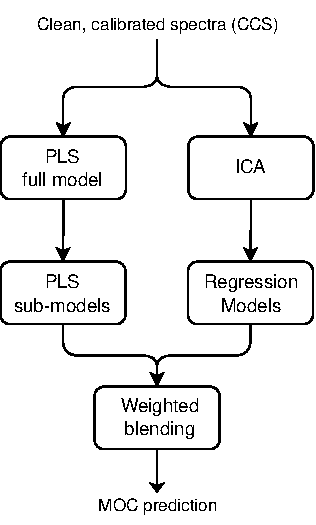
\includegraphics[width=0.225\textwidth]{images/moc_pipeline.pdf}
	\caption{Overview of the \gls{moc} model.}
	\label{fig:moc_pipeline}
\end{figure}

In \citet{p9_paper}, we presented our efforts to replicate the \gls{moc} model.
Based on the insights gained from that work, we have made several modifications to the replica in preparation for this work.

Our replica only utilized a single dataset for the \gls{ica} phase, while the original model used all five datasets.
This difference was due to the original paper not specifying how the five datasets were used, and so we designed an experiment to determine how to use them in a way that would most closely replicate the original model.
We initially assumed that the datasets were aggregated and used as a single dataset.
This approach, however, did not align with the original model's results, likely due to the loss of information from the individual datasets.
Following this discovery, we modified the replica to instead use the datasets in the same way as in the \gls{pls1-sm} phase, which yielded results aligning more closely with the original model.

Furthermore, our initial replica used a random train/test split for training, in contrast to the original model's manual curation to ensure representation of extreme compositions in both sets.
This difference stemmed from the original authors' application of domain expertize in their dataset curation --- a process we could not directly replicate.
Nevertheless, we found that automatically identifying extreme compositions and ensuring that they were present in both the training and testing sets brought us closer to the original model.
We chose to pull out the $n$ largest and smallest samples by concentration range, for each oxide, and reserve them for the training set.
Then we would do a random split on the remaining dataset, such that the final train/test split would be a $80\%/20\%$ split.

With these changes, we created a more accurate replica of the \gls{moc} model, which we will use as our baseline for the rest of this paper.
We have presented these changes to one of the original authors of~\citet{cleggRecalibrationMarsScience2017}, who confirmed that they were reasonable and in line with the original model's implementation.

Table~\ref{tab:replica_results_rmses} shows the \gls{rmse}s of the original models and our replicas after the changes.
Figure~\ref{fig:rmse_histograms} illustrates the distribution of these \gls{rmse}s as a grouped histogram.
The results show that the \gls{rmse}s of our replicas exhibit similar tendencies to the original models.
However, in some cases, our replicas have a lower \gls{rmse} than the original models, and in others, they have a higher \gls{rmse}.
These differences are due to a number of factors.

Firstly, the original models were trained with datasets from 1600mm and 3000mm standoff distances~\cite{cleggRecalibrationMarsScience2017}, while we only had access to the 1600mm dataset for our replicas.
Additionally, we automated the outlier removal for the PLS1-SM phase, unlike the original manual process.
As mentioned, the original authors manually curated their training and test sets, ensuring a broad elemental range, while we implemented an automatic process for our replicas due to lack of domain expertise.
Differences might also stem from varied implementation specifics, such as programming languages and libraries used.

\begin{table*}
	\centering
	\begin{tabular*}{\textwidth}{@{\extracolsep{\fill}}lllllll}
		\hline
		Element    & \gls{pls1-sm} (original) & PLS1-SM (replica) & \gls{ica} (original) & ICA (replica) & \gls{moc} (original) & \gls{moc} (replica) \\
		\hline
		\ce{SiO2}  & 4.33                     & 4.52              & 8.31                 & 8.63          & 5.30                 & 5.61                \\
		\ce{TiO2}  & 0.94                     & 0.49              & 1.44                 & 0.54          & 1.03                 & 0.61                \\
		\ce{Al2O3} & 2.85                     & 1.79              & 4.77                 & 3.18          & 3.47                 & 2.47                \\
		\ce{FeO_T} & 2.01                     & 2.16              & 5.17                 & 2.87          & 2.31                 & 1.82                \\
		\ce{MgO}   & 1.06                     & 0.91              & 4.08                 & 3.11          & 2.21                 & 1.56                \\
		\ce{CaO}   & 2.65                     & 1.73              & 3.07                 & 3.28          & 2.72                 & 2.09                \\
		\ce{Na2O}  & 0.62                     & 0.80              & 2.29                 & 1.39          & 0.62                 & 1.33                \\
		\ce{K2O}   & 0.72                     & 0.72              & 0.98                 & 1.38          & 0.82                 & 1.91                \\
		\hline
	\end{tabular*}
	\caption{\gls{rmse}s of the original and our replicas of the \gls{pls1-sm}, \gls{ica}, and \gls{moc} models.}
	\label{tab:replica_results_rmses}
\end{table*}

\begin{figure*}
	\centering
	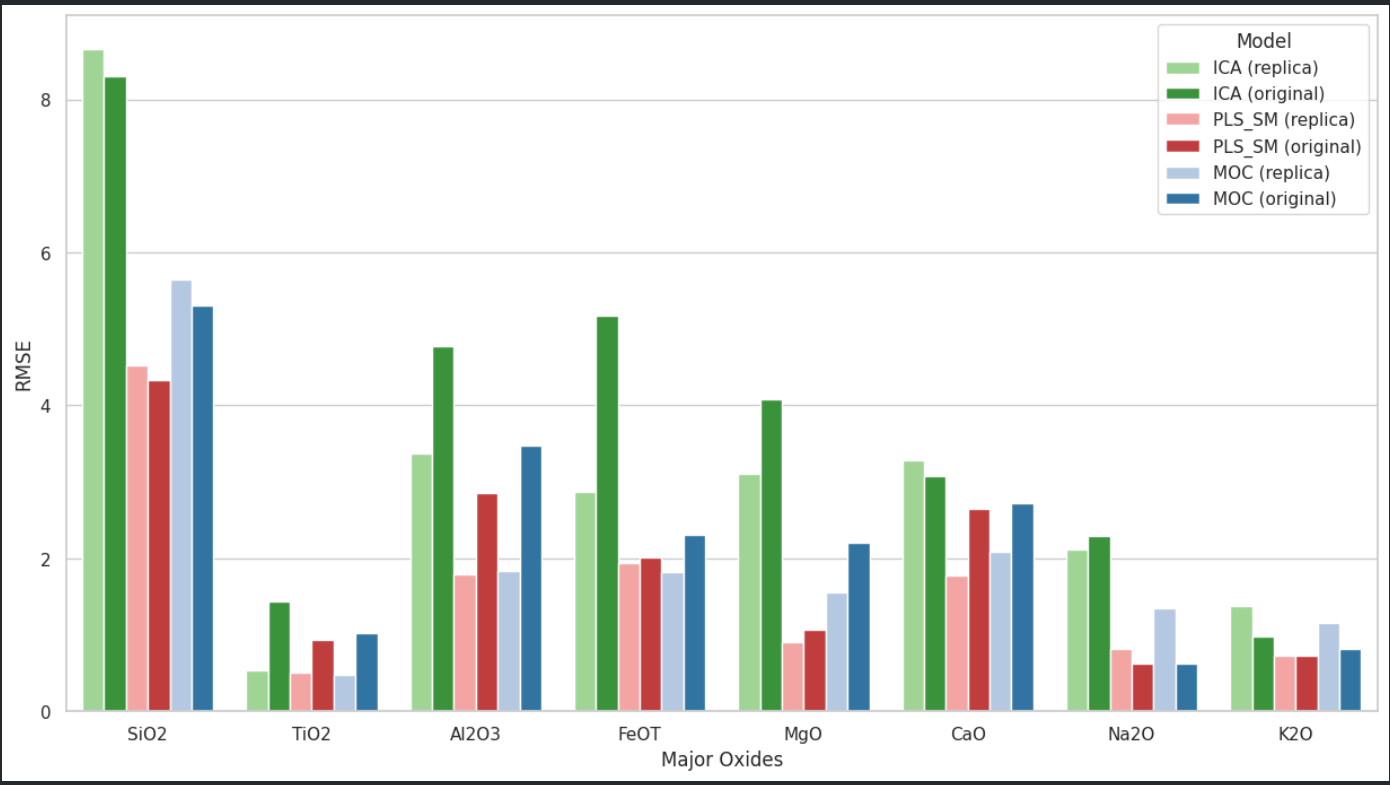
\includegraphics[width=0.85\textwidth]{images/rmse_historgram.png}
	\caption{Grouped histogram of the \gls{rmse}s of the original and our replicas of the \gls{pls1-sm}, \gls{ica}, and \gls{moc} models.}
	\label{fig:rmse_histograms}
\end{figure*}

Through a series of comparative experiments, we showed that the model selection was the primary cause of these limitations, and we showed how both \gls{ann} and \gls{gbr} methods could be used to improve the model's predictive accuracy and robustness.
This is further underscored by work from the SuperCam team.
In 2021, the Perseverance rover landed on Mars, equipped with the SuperCam instrument, which is the successor to the \gls{chemcam} instrument.
As part of the ongoing work to support the SuperCam instrument, \citet{andersonPostlandingMajorElement2022} experimented with various machine learning models to predict the composition of major oxides in geological samples using the SuperCam \gls{libs} calibration dataset.
While the team decided to retain \gls{pls} for analyzing certain oxides, \gls{ica} was entirely discontinued.
Instead, models based on \gls{gbr}, \gls{rf}, and \gls{lasso} were selected for other oxides.
This decision reinforces our finding that \gls{ica} regression models fall short in accurately predicting the composition of major oxides in geological samples.
Consistent with our observations, \gls{gbr} was also identified as a high-performing model in their analyses.

\subsection{Data Normalization}\label{sec:data_normalization}
The \gls{chemcam} instrument consists of three spectrometers, each producing 2048 channels.
For data normalization, we follow the approach taken by the SuperCam team and normalize across individual spectrometers' wavelength ranges, a process known as \textit{Norm 3}~\cite{andersonPostlandingMajorElement2022}.
This method ensures that the wavelength intensities captured by each spectrometer is normalized independently.

Figure~\ref{fig:spectral_plot} shows a spectral plot of the \gls{ccs} data for the \textit{ultramafic} sample, illustrating the three distinct spectral regions, each captured by one of the three spectrometers. Specifically, one spectrometer captures the \gls{uv} region, another captures the \gls{vio} region, and the third captures the \gls{vnir} region.

\begin{figure}[H]
	\centering
	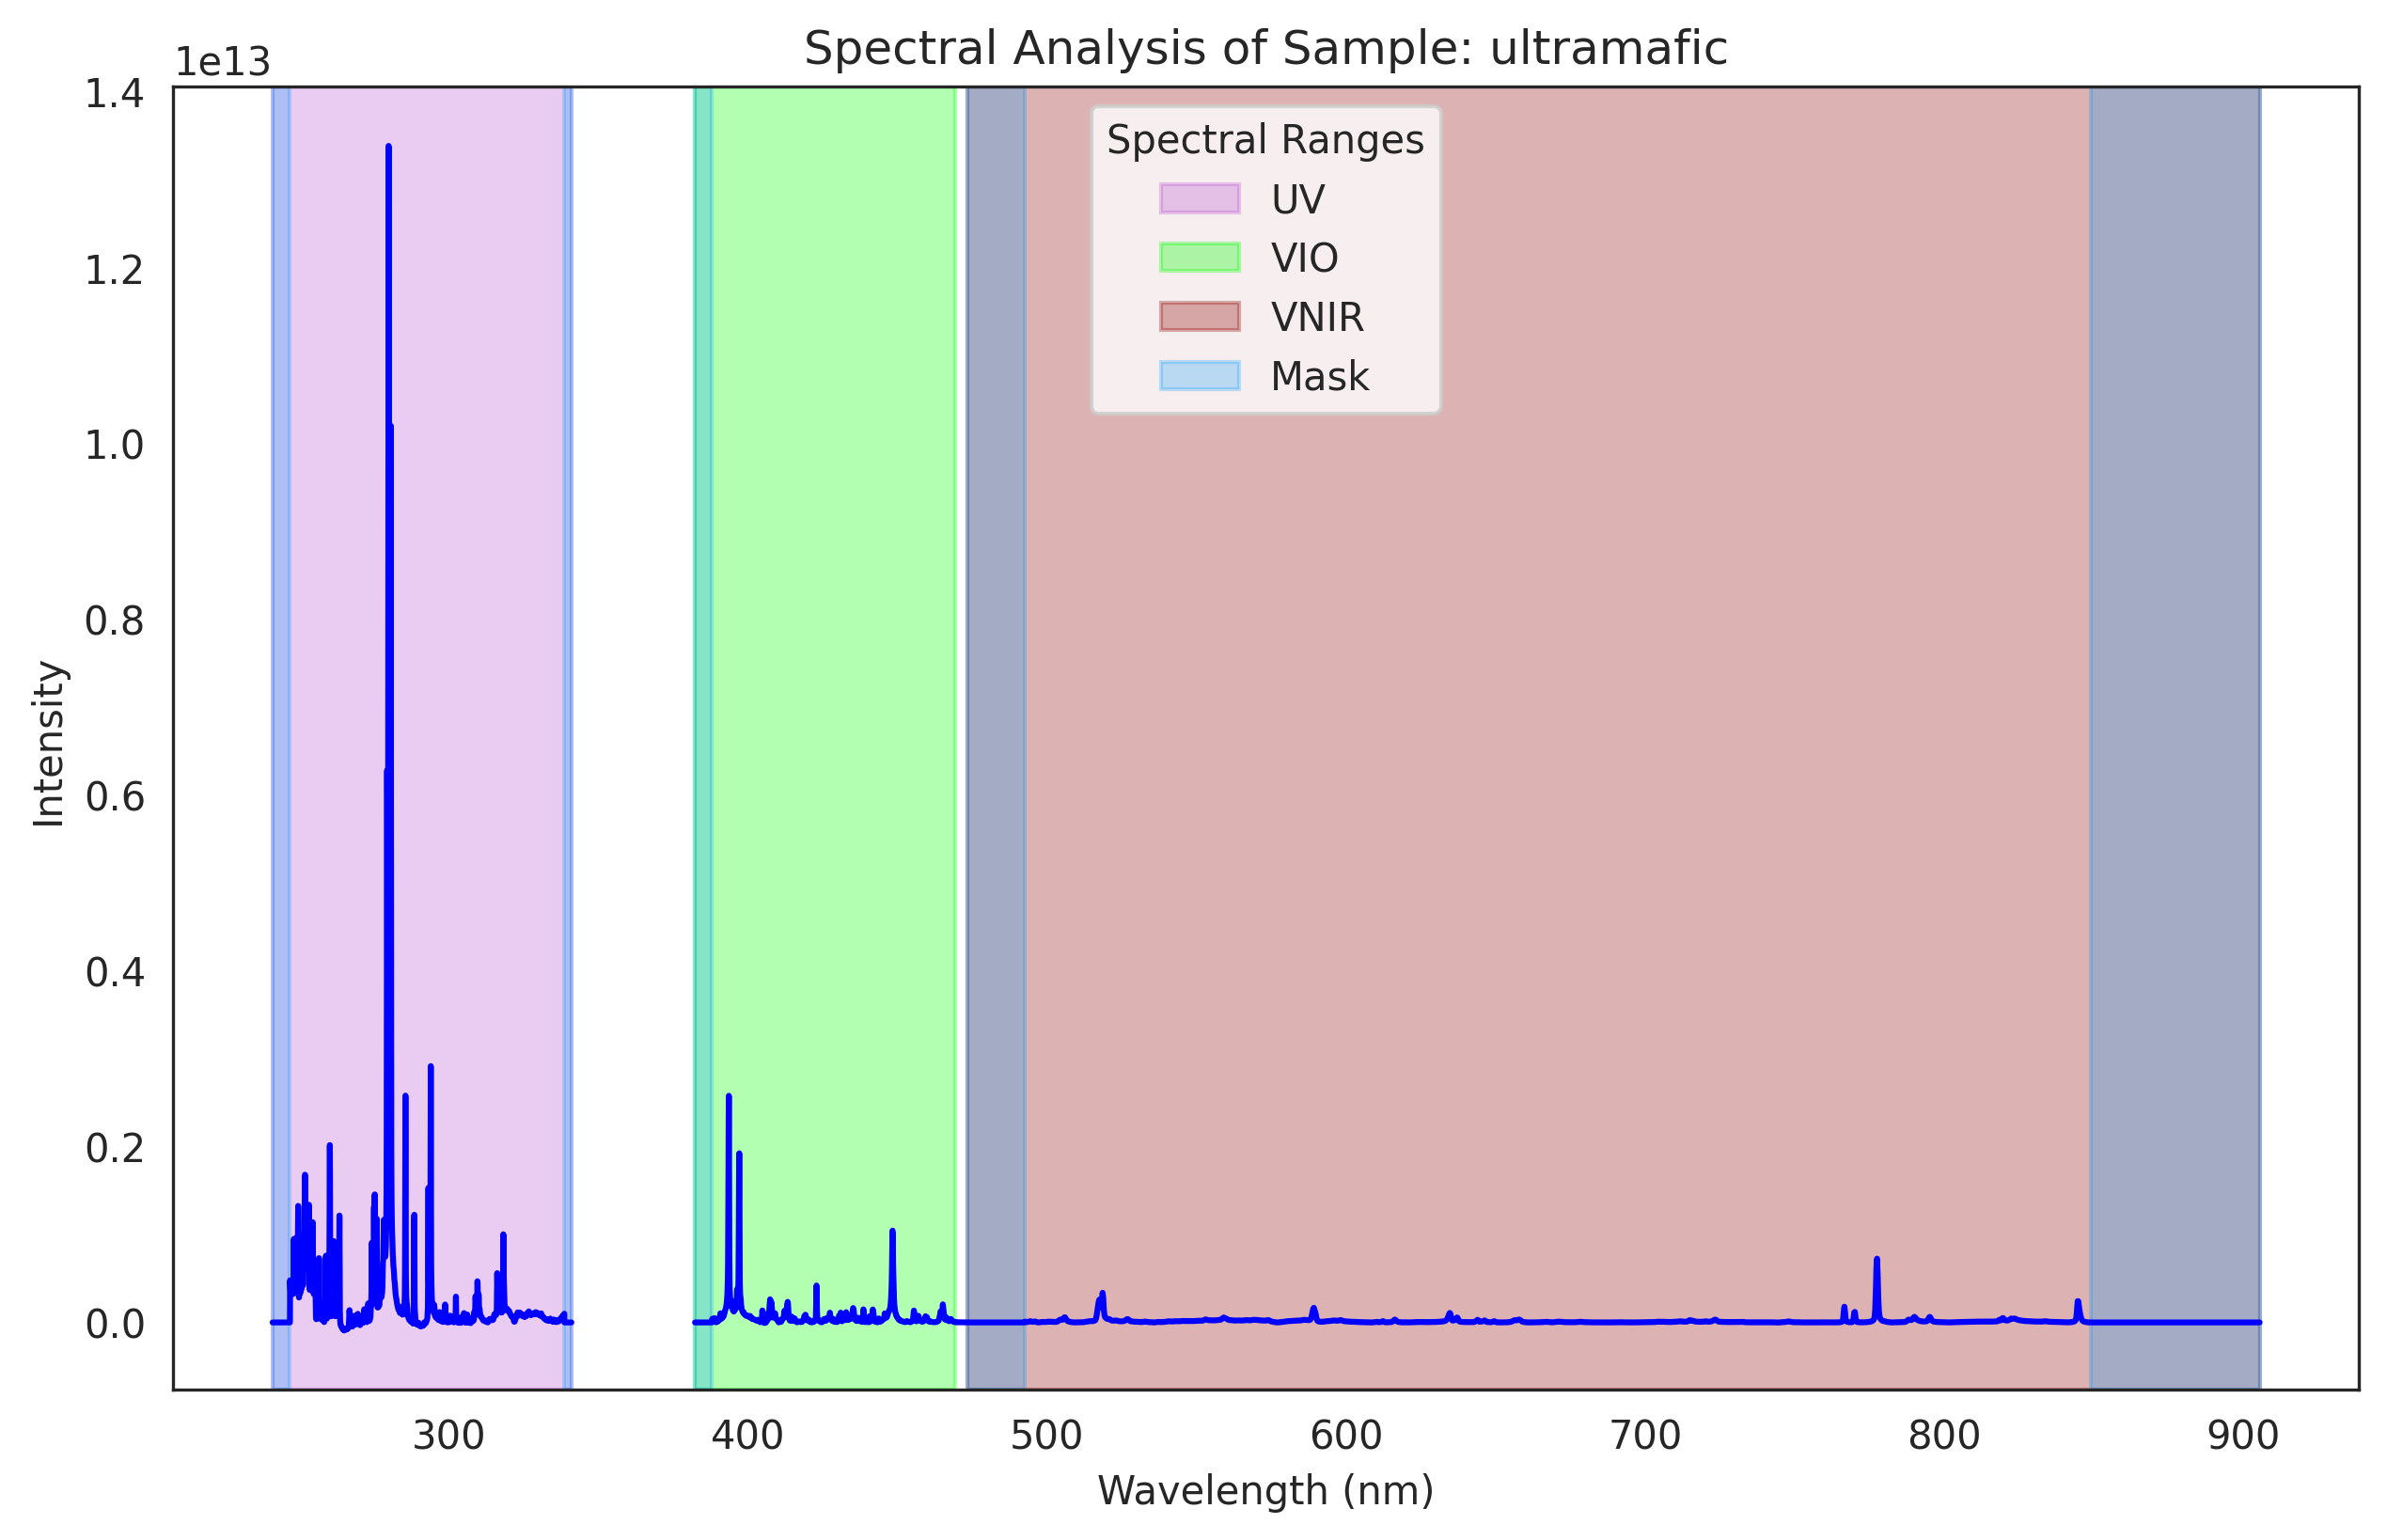
\includegraphics[width=0.5\textwidth]{images/spectral_plot.png}
	\caption{Spectral plot of the \gls{ccs} data for the \textit{ultramafic} sample. The wavelengths represent the spectral channels.}
	\label{fig:spectral_plot}
\end{figure}

Norm 3 can be understood as follows: for each sample, we consider the data from each spectrometer separately. Within each spectrometer, we divide the intensity of each channel by the sum of all channel intensities for that spectrometer. This process is applied for all three spectrometers, resulting in normalized data that preserves the relative intensities within each spectrometer while allowing for comparisons across different samples.

Formally, Norm 3 is defined as

\begin{equation}
	\tilde{X}_{i,j}^{(s)} = \frac{X_{i,j}^{(s)}}{\sum_{j=1}^{N} X_{i,j}^{(s)}},
\end{equation}

where

\begin{itemize}
	\item $\tilde{X}_{i,j}^{(s)}$ is the normalized wavelength intensity for the $i$-th sample in the $j$-th channel on the $s$-th spectrometer with $s \in \{1, 2, 3\}$,
	\item $X_{i,j}^{(s)}$ is the original wavelength intensity for the $i$-th sample in the $j$-th channel on the $s$-th spectrometer,
	\item $N = 2048$ is the number of channels in each spectrometer, and
\end{itemize}

This normalization method results in a total of $3N = 6144$ normalized features for each sample, as each of the three spectrometers contributes 2048 channels.

\subsection{Overview of Core Models}
In this section, we provide an overview and definitions of \gls{pls}, primarily based on the methodologies described by \citet{James2023AnIS}.
These models form the basis of the final architecture of our proposed pipeline, detailed further in Section~\ref{sec:methodology}.

\subsubsection{PLS}
To understand \gls{pls}, it is essential to first understand \gls{pca} and \gls{pcr}.

\gls{pca} is a dimensionality reduction technique that transforms a set of possibly correlated variables into a smaller set of uncorrelated variables called \textit{principal components}.
First, the data matrix $\mathbf{X}$ is centered by subtracting the mean of each variable to ensure that the data is centered at the origin:

$$
\mathbf{\bar{X}} = \mathbf{X} - \mathbf{\mu},
$$

where $\mathbf{\bar{X}}$ is the centered data matrix and $\mathbf{\mu}$ is the mean of each variable.

The covariance matrix of the centered data is then computed:

$$
\mathbf{C} = \frac{1}{n-1} \mathbf{\bar{X}}^T \mathbf{\bar{X}},
$$

where $n$ is the number of samples.

Then, the covariance matrix $C$ is decomposed into its eigenvectors $\mathbf{V}$ and eigenvalues $\mathbf{D}$:

$$
\mathbf{C} = \mathbf{V} \mathbf{D} \mathbf{V}^T,
$$

where matrix $\mathbf{V}$ contains the eigenvectors of $\mathbf{C}$ and represents the principal component loadings.
These loadings indicate the directions of maximum variance in $\mathbf{X}$.
The matrix $\mathbf{D}$ is diagonal and holds the eigenvalues, each of which quantifies the variance captured by its corresponding loading.

These components are the scores $\mathbf{T}$, calculated as follows:

$$
\mathbf{T} = \mathbf{\bar{X}} \mathbf{V}_n,
$$

where $\mathbf{V}_n$ includes only the top $n$ eigenvectors.
The scores $\mathbf{T}$ are the new, uncorrelated features that reduce the dimensionality of the original data, capturing the most significant patterns and trends.

Finally, the original data points are projected onto the space defined by the top $n$ principal components, which transforms $X$ into a lower-dimensional representation:

$$
\mathbf{X}_{\text{reduced}} = \mathbf{\bar{X}} \mathbf{V}_n,
$$

where $\mathbf{V}_n$ is the matrix that only contains the top $n$ eigenvectors.

\gls{pcr} extends \gls{pca} in the context of regression analysis.
First, \gls{pca} is applied to the dataset $\mathbf{X}$, transforming it into a set of uncorrelated variables, the principal components.
These components, represented by scores $\mathbf{T}$, are derived from the eigenvectors $\mathbf{V}_n$ with the highest variances.

In \gls{pcr}, the dataset $\mathbf{X}$ is decomposed using PCA as:

$$
\mathbf{X} = \mathbf{TV}^T + \mathbf{E},
$$

where $\mathbf{T}$ represents the scores, and $\mathbf{V}$ represents the loadings.
\gls{pcr} utilizes these scores $\mathbf{T}$ in a linear regression model to predict the target variable $\mathbf{y}$:

$$
\mathbf{y} = \mathbf{Tb} + \mathbf{e},
$$

where $\mathbf{b}$ are the regression coefficients correlating $\mathbf{T}$ to $\mathbf{y}$, and $\mathbf{e}$ is the vector of residuals, capturing the prediction errors.

However, one drawback of \gls{pcr} is that it does not consider the target in the decomposition of the features and therefore assumes that smaller components have a weaker correlation with the target than the larger ones.
This assumption does not always hold, which is what \gls{pls} aims to address.

\gls{pls} uses an iterative method to identify components that maximize the covariance between the features and the target.m
These components, $Z$, are linear combinations of the original features, $X_j$, weighted by coefficients, $\phi_j$, which are specifically calculated to reflect this covariance.
The formula for each component is expressed as:

$$
    Z = \sum_{j=1}^{p} \phi_j X_j,
$$

where $Z$ represents the component, $X_j$ is the $j$-th feature, and $\phi_j$ is the weight for the $j$-th feature.
The weights, $\phi_j$, are determined by the formula:

$$
    \phi_j = \frac{\text{cov}(X_j, Y)}{\text{var}(X_j)}.
$$

To refine the model iteratively, PLS uses the residuals from the previous components to calculate the next component.
The $m$-th component, for example, is derived from the residuals of the previous $m-1$ components:

$$
    Z_m = \sum_{j=1}^{p} \phi_{jm} \hat{X}_{j, m-1}.
$$

The components are then used to predict the target variable by fitting a linear model via least squares regression.
